\documentclass{article}
\usepackage{amsmath}
\usepackage{enumitem}
\usepackage[margin=0.5in]{geometry}
\usepackage{listings}
\usepackage{tikz}
\usepackage{hyperref}

\title{COMP3520 Assignment 1}
\author{Brandon Lucier - 104516782}

\begin{document}

\maketitle

\begin{enumerate}
    \item{
        Using the C language a structure to define a pixel and an array of $M * N$ pixels would be:
        
        \begin{lstlisting}[language=C]
struct Pixel {
    unsigned char red;
    unsigned char green;
    unsigned char blue;
};
    
struct Pixel DISPLAY[M * N];
        \end{lstlisting}
        
        The point \textbf{P=(X, Y)} would be located at offset $y * N + x$ from \&DISPLAY.
        
        For example:
        
        \begin{lstlisting}[language=C]
struct Pixel* p = DISPLAY + y * N + x;
p->red = 255;
        \end{lstlisting}
    }
    \item{
        Screen dimensions: 29.44cm x 16.56cm\\
        Resolution: 1920 x 1080\\
        $29.44 / 1920 = 0.01534$\\
        $16.56 / 1080 = 0.01534$\\
        The distance between pixels is 0.1534mm.
        
        The smallest objects the human eye can see is about 0.1mm.
        
        \url{https://learn.genetics.utah.edu/content/cells/scale/}
    }
    \item{
        \begin{enumerate}[label=\alph*.]
            \item {
                $P_{1} = (-3, 4)$\\
                $P_{2} = (4, -2)$
                
                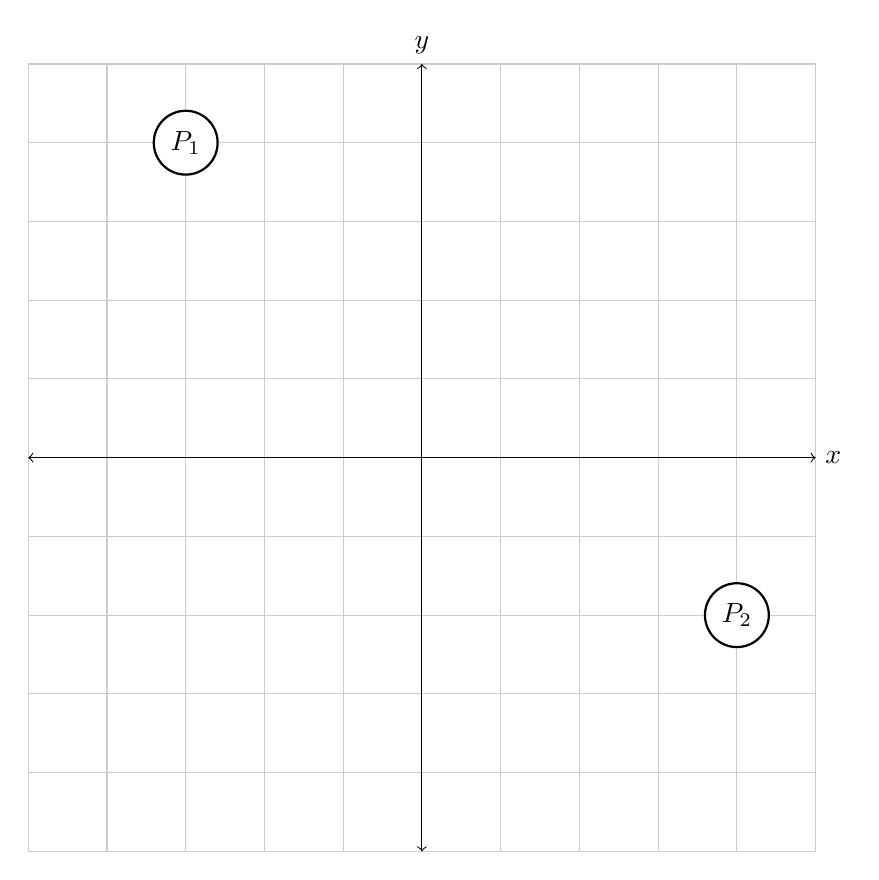
\begin{tikzpicture}[place/.style={circle,draw=black,fill=white,thick}]
                      \draw[thin,gray!40] (-5,-5) grid (5,5);
                      \draw[<->] (-5,0)--(5,0) node[right]{$x$};
                      \draw[<->] (0,-5)--(0,5) node[above]{$y$};
                      \node (n1) at (-3,4) [place] {$\small{P_{1}}$};
                      \node (n1) at (4,-2) [place] {$\small{P_{2}}$};
                \end{tikzpicture}
            }
            \item {
                $P_{1} = (1, -3)$\\
                $P_{2} = (-2, 2)$
                
                $V_{1} = P_{1} - P{2} = \begin{bmatrix} 1 - (-2) \\ -3 - 2 \end{bmatrix} = \begin{bmatrix} 3 \\ -5 \end{bmatrix}$\\
                $V_{2} = P_{2} - P{1} = \begin{bmatrix} -2 - 1 \\ 2 - (-3) \end{bmatrix} = \begin{bmatrix} -3 \\ 5 \end{bmatrix}$
            
                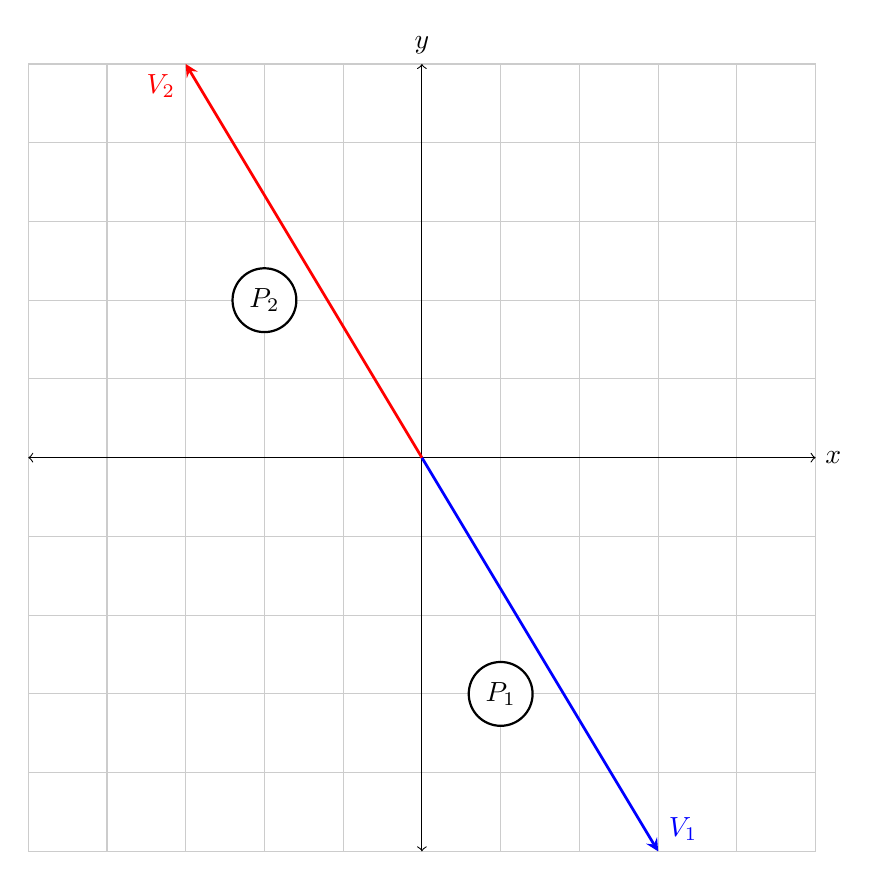
\begin{tikzpicture}[place/.style={circle,draw=black,fill=white,thick}]
                      \draw[thin,gray!40] (-5,-5) grid (5,5);
                      \draw[<->] (-5,0)--(5,0) node[right]{$x$};
                      \draw[<->] (0,-5)--(0,5) node[above]{$y$};
                      
                      \draw[line width=1pt,blue,-stealth](0,0)--(3,-5) node[anchor=south west]{$V_{1}$};
                      \draw[line width=1pt,red,-stealth](0,0)--(-3,5) node[anchor=north east]{$V_{2}$};
                      
                      \node (n1) at (1,-3) [place] {$\small{P_{1}}$};
                      \node (n1) at (-2,2) [place] {$\small{P_{2}}$};
                \end{tikzpicture}
                
                The two vectors $V_{1}$ and $V_{2}$ are mirrors of each other. Adding them together will give a vector of $\begin{bmatrix} 0 \\ 0 \end{bmatrix}$. Adding $V_{2}$ to $P_{1}$ will give $P_{2}$ and adding $V_{1}$ to $P_{2}$ will give $P_{1}$.
            }
            \item {
                The dot product of the vector $V_{1} = \begin{bmatrix} 2 \\ 5 \end{bmatrix}$ and the vector $V_{2} = \begin{bmatrix} -3 \\ 4 \end{bmatrix}$ can be solved as follows:
                
                $V_{1} \cdot V_{2} = \begin{bmatrix} 2 \\ 5 \end{bmatrix} \cdot \begin{bmatrix} -3 \\ 4 \end{bmatrix} = (2 \times -3) + (5 \times 4) = 14$
                
                There is no difference between $V_{1} \cdot V_{2}$ and $V_{2} \cdot V_{1}$ because the dot product is commutative.
                
                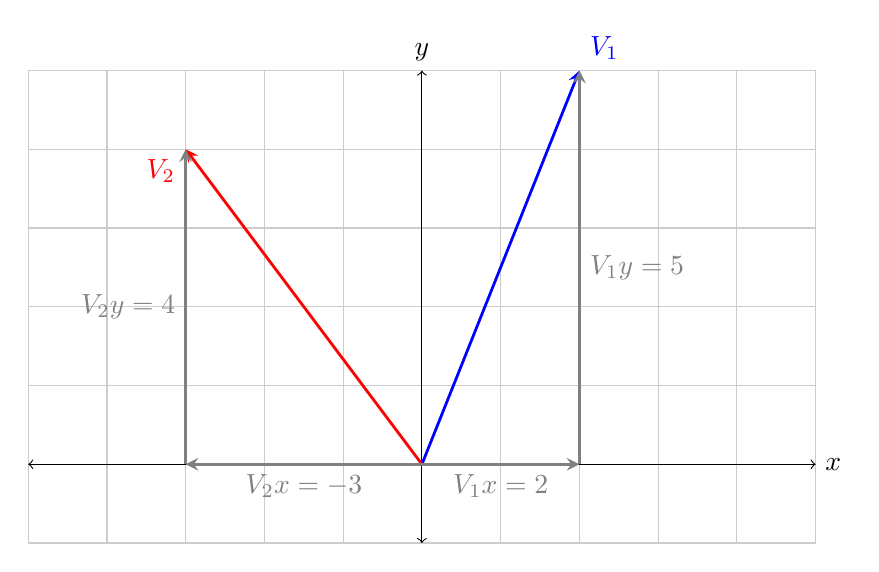
\begin{tikzpicture}
                      \draw[thin,gray!40] (-5,-1) grid (5,5);
                      \draw[<->] (-5,0)--(5,0) node[right]{$x$};
                      \draw[<->] (0,-1)--(0,5) node[above]{$y$};
                      
                      \draw[line width=1pt,blue,-stealth](0,0)--(2,5) node[anchor=south west]{$V_{1}$};
                      \draw[line width=1pt,red,-stealth](0,0)--(-3,4) node[anchor=north east]{$V_{2}$};
                      
                      \draw[line width=1pt,gray,-stealth](2,0)--(2,5) node[midway, right]{$V_{1}y = 5$};
                      \draw[line width=1pt,gray,-stealth](0,0)--(2,0) node[midway, below]{$V_{1}x = 2$};
                      
                      \draw[line width=1pt,gray,-stealth](-3,0)--(-3,4) node[midway, left]{$V_{2}y = 4$};
                      \draw[line width=1pt,gray,-stealth](0,0)--(-3,0) node[midway, below]{$V_{2}x = -3$};
                \end{tikzpicture}
            }
            \item {
                $V_{1} = \begin{bmatrix} 2 \\ 4 \\ 6 \end{bmatrix}$\\
                $V_{2} = \begin{bmatrix} 3 \\ 5 \\ 7 \end{bmatrix}$
                
                \begin{enumerate}[label=\roman*.]
                    \item {
                        $
                            V_{1} - V_{2}  = 
                            \begin{bmatrix}
                                2 - 3 \\
                                4 - 6 \\
                                6 - 7
                            \end{bmatrix}
                            =
                            \begin{bmatrix}
                                -1 \\ -1 \\ -1
                            \end{bmatrix}
                        $
                    }
                    \item {
                        $\lvert V_{1} \rvert = \sqrt{2^{2} + 4^{2} + 6^{2}} = \sqrt{56}$\\
                        $\lvert V_{2} \rvert = \sqrt{3^{2} + 5^{2} + 7^{2}} = \sqrt{83}$
                    }
                    \item {
                        $
                        V_{1} \cdot V_{2} = 
                        \begin{bmatrix} 2 \\ 4 \\ 6 \end{bmatrix} 
                        \cdot 
                        \begin{bmatrix} 3 \\ 5 \\ 7 \end{bmatrix}
                        =
                        2(3) + 4(5) + 6(7) = 68
                        $
                    }
                    \item {
                        $
                        V_{1} \times V_{2} =
                        \begin{bmatrix} 2 \\ 4 \\ 6 \end{bmatrix}
                        \times
                        \begin{bmatrix} 3 \\ 5 \\ 7 \end{bmatrix}
                        =
                        \begin{bmatrix}
                        4(7) - 6(5) \\
                        6(3) - 2(7) \\
                        2(5) - 4(3)
                        \end{bmatrix}
                        =
                        \begin{bmatrix} -2 \\ 4 \\ 2 \end{bmatrix}
                        $\\
                        $
                        V_{2} \times V_{1} = 
                        \begin{bmatrix} 3 \\ 5 \\ 7 \end{bmatrix}
                        \times
                        \begin{bmatrix} 2 \\ 4 \\ 6 \end{bmatrix}
                        =
                        \begin{bmatrix}
                        5(6) - 7(4) \\
                        7(2) - 3(6) \\
                        3(4) - 5(2)
                        \end{bmatrix}
                        =
                        \begin{bmatrix}
                        2 \\
                        -4 \\
                        2
                        \end{bmatrix}
                        $
                    }
                \end{enumerate}
            }
        \end{enumerate}
    }
    
    \item {
        $
        M_{1} =
        \begin{bmatrix}
        1 & 3 & -2 \\
        2 & -1 & 4
        \end{bmatrix}
        $
        
        $
        M_{2} = 
        \begin{bmatrix}
        1 & 2 & 1/2 \\
        -1/2 & -1 & 1 \\
        0 & 1 & 2
        \end{bmatrix}
        $
        
        \begin{enumerate}[label=\roman*.]
            \item {
                The inverse matrix $M_{1}^{-1}$ does not exist because it is not a square matrix.
                
                The inverse matrix $M_{2}^{-1}$ can be found as follows:
                
                Create a matrix of minors for $M_{2}$:
                
                $
                \begin{bmatrix}
                (-1)(2) - (1)(1) & (-1/2)(2) - (1)(0) & (-1/2)(1) - (-1)(0) \\
                (2)(2) - (1/2)(1) & (1)(2) - (1/2)(0) & (1)(1) - (2)(0) \\
                (2)(1) - (1/2)(-1) & (1)(1) - (1/2)(-1/2) & (1)(-1) - (2)(-1/2)
                \end{bmatrix}
                =
                \begin{bmatrix}
                -3  & -1 & -1/2 \\
                7/2 & 2 & 1 \\
                5/2 & 5/4 & 0
                \end{bmatrix}
                $
                
                Create a matrix of co-factors:
                
                $
                \begin{bmatrix}
                -3 & 1 & -1/2 \\
                -7/2 & 2 & -1 \\
                5/2 & -5/4 & 0
                \end{bmatrix}
                $
                
                Transpose that matrix:
                
                $
                \begin{bmatrix}
                -3 & -7/2 & 5/2 \\
                1 & 2 & -5/4 \\
                -1/2 & -1 & 0
                \end{bmatrix}
                $
                
                Multiply the matrix by the determinant of the original matrix:
                
                $
                \det M_{2} =
                1((-1)(2) - (1)(1)) -
                2((-1/2)(2) - (1)(0)) + 
                (1/2)((-1/2)(1) - (-1)(0))
                = -4/5
                $
                
                $
                M_{2}^{-1} = 
                -4/5
                \begin{bmatrix}
                -3 & -7/2 & 5/2 \\
                1 & 2 & -5/4 \\
                -1/2 & -1 & 0
                \end{bmatrix}
                =
                \begin{bmatrix}
                12/5 & 14/5 & -2 \\
                -4/5 & -8/5 & 1 \\
                -2/5 & 4/5 & 0
                \end{bmatrix}
                $
            }
            
            \item {
                $
                M_{1}^{T} = 
                \begin{bmatrix}
                1 & 2 \\
                3 & -1 \\
                -2 & -4
                \end{bmatrix}
                $
            
                $
                M_{2}^{T} =
                \begin{bmatrix}
                1 & -1/2 & 0 \\
                2 & -1 & 1 \\
                1/2 & 1 & 2
                \end{bmatrix}
                $
            }
            
            \item {
                The determinant $\det M_{1}$ does not exist because it is not a square matrix.
                
                $
                \det M_{2} =
                1((-1)(2) - (1)(1)) -
                2((-1/2)(2) - (1)(0)) + 
                (1/2)((-1/2)(1) - (-1)(0))
                = -4/5
                $
            }
            
            \item {
                $
                M_{1} \cdot M_{2} =
                \begin{bmatrix}
                1 & 3 & -2 \\
                2 & -1 & 4
                \end{bmatrix}
                \cdot
                \begin{bmatrix}
                1 & 2 & 1/2 \\
                -1/2 & -1 & 1 \\
                0 & 1 & 2
                \end{bmatrix}
                $
                
                $
                M_{11} = (1)(1) + (3)(-1/2) + (-2)(0) = -1/2 \\
                M_{12} = (1)(2) + (3)(-1) + (-2)(1) = -3 \\
                M_{13} = (1)(1/2) + 3(1) + (-2)(2) = -1/2 \\ \\
                M_{21} = (2)(1) + (-1)(-1/2) + (4)(0) = 5/2 \\
                M_{22} = (2)(2) + (-1)(-1) + (4)(1) = 9 \\
                M_{23} = (2)(1/2) + (-1)(1) + (4)(2) = 8 \\ \\
                M_{1} \cdot M_{2} = 
                \begin{bmatrix}
                M_{11} & M_{12} & M_{13} \\
                M_{21} & M_{22} & M_{23}
                \end{bmatrix}
                =
                \begin{bmatrix}
                -1/2 & -3 & -1/2 \\
                5/2 & 9 & 8
                \end{bmatrix}
                $
            }
            
            \item {
            No the inner product or $M_{1}$ and $M_{2}$ is not commutative. The inner dimensions of the two matrices would not be the same.
            }
        \end{enumerate}
    
    }
\end{enumerate}

\end{document}
